\settitle[Duqu contre Duqu]{Duqu contre Duqu : Analyse et détournement du driver de Duqu}

% \documentclass[times,11pt,fullpage]{article}

% \usepackage{amssymb} % not included
% \usepackage{graphicx} % included
% \usepackage[utf8x]{inputenc} % not included
% \usepackage{url,hyperref} % not included
% \usepackage{fullpage} % not included
% \usepackage{float} %not included
% \usepackage{framed} %not included
% \usepackage{francais} %included
% \usepackage{wrapfig} %not included

%%%% debut macro %%%%
\newenvironment{changemargin}[2]{\begin{list}{}{%
\setlength{\topsep}{0pt}%
\setlength{\leftmargin}{0pt}%
\setlength{\rightmargin}{0pt}%
\setlength{\listparindent}{\parindent}%
\setlength{\itemindent}{\parindent}%
\setlength{\parsep}{0pt plus 1pt}%
\addtolength{\leftmargin}{#1}%
\addtolength{\rightmargin}{#2}%
}\item }{\end{list}}
%%%% fin macro %%%%

% Duqu modules
\newcommand{\Crysys}{\texttt{CrySys}}
\newcommand{\Duqu}{\texttt{Duqu}}
\newcommand{\Stuxnet}{\texttt{Stuxnet}}
\newcommand{\driver}{\texttt{nfrd965.sys}}
\newcommand{\netpDLL}{\texttt{NETP191.PNF}}
\newcommand{\cmiDLL}{\texttt{CMI4432.PNF}}
\newcommand{\netpCONF}{\texttt{netp192.PNF}}
\newcommand{\cmiCONF}{\texttt{CMI4464.PNF}}
\newcommand{\jminet}{\texttt{JMINET7.SYS}}
\newcommand{\cmi}{\texttt{CMI4432.SYS}}
\newcommand{\krn}{\texttt{kernel.dll}}
% windows stuff
\newcommand{\service}{\texttt{services.exe}}

% Pas besoin d'obfusquer les adresses mails, \email s'en chargera (XXX)
\setauthor[G.~Bonfante, J-Y.~Marion, F.~Sabatier, A.~Thierry]{Guillaume Bonfante, Jean-Yves Marion, Fabrice Sabatier et Aurélien~Thierry	\\
  \email{prenom.nom@loria.fr}}

% XXX: Gérer le cas des compagnies multiples
\institute{LORIA, Inria, Université de Lorraine}

\maketitle
\index{MonNom7, M.}
\index{MonAutreNom8, A.}

\begin{abstract}
Proche de \Stuxnet\ avec lequel il partage des fonctionnalités, \Duqu\ a fait l'objet de nombreuses analyses au cours de l'année passée. Nous nous proposons d'en étudier un élément en particulier, le driver. Notre contribution consiste en la rétroingénierie de ce composant par la reconstitution de son code source et une analyse de ses fonctionnalités. Nous avons ensuite détourné le driver pour détecter d'éventuelles injections dans les exécutables Windows et prévenir d'autres attaques. En particulier nous montrons comment le driver de \Duqu\ modifié aurait permis de détecter \Duqu.
\end{abstract}

%% Découpage en sections
%% =====================
%% 
%% La classe llcns ne définit que 4 niveaux de sections :
%% 
%% * section
%% * subsection
%% * subsubsection
%% * paragraph
%% 

\section{Introduction}

Lors de sa découverte en septembre 2011 par \Crysys, laboratoire de sécurité et de cryptographie de l'université de Budapest \cite{AThierry_CrysysDuquStuxnet}, il a été dit de \Duqu, un malware d'espionnage, qu'il était apparenté à un autre code malveillant : \Stuxnet. L'argument tient au fait que les deux malware emploient les \emph{mêmes} mécanismes pour assurer leur primo-infection ; or, la sophistication même de ces mécanismes est une signature de leurs auteurs, et donc lie les deux attaques. Mais l'adage veut que les systèmes complexes soient fragiles. Nous  illustrons ici ce principe en détournant les fonctionnalités de \Duqu\ pour en faire un système de détection d'injection de code, rudimentaire mais capable de détecter une attaque par Duqu.


\Duqu\ est un outil offensif utilisé pour le vol d'informations. Symantec \cite{AThierry_SymantecDuqu2011} a identifié parmi les fonctionnalités de \Duqu\ des enregistreurs de frappes (\emph{keylogger}), de l'écran, de l'activité réseau, des programmes ouverts, ainsi des outils de découverte de services. Le malware est maintenu à jour via un serveur de Command \& Control. Il est également muni d'un mécanisme d'auto-destruction après 36 jours s'il n'a pas reçu de notification contraire du C\&C. 
Les attaques semblent réussies puisque le malware n'a pas été détecté à chaud alors que certaines opérations ont duré plusieurs mois, mais seulement "post-mortem".
De nombreuses souches du malware ont été trouvées dans la nature, chacune avec des binaires différents mais similaires. Kasperky a fait un bon historique des versions \cite{AThierry_KaspDuqu10}, la dernière souche détectée datant de février 2012 alors que \Duqu\ était déjà largement découvert et documenté.
En résumé, \Duqu\ est un logiciel espion, discret, s'adaptant spécifiquement à sa cible. 

Or, nous développons au Laboratoire de Haute Sécurité du LORIA, un prototype de détecteur de virus fondé sur l'analyse morphologique~\cite{AThierry_BKM08}, technique basée sur la comparaison des graphes de flot de contrôle.  Dès que nous avons eu les échantillons de \Stuxnet\ et \Duqu, nous avons cherché à savoir si notre méthode --connaissant \Stuxnet-- aurait permis de détecter l'attaque de \Duqu. De fait, la réponse est \emph{positive} si nous disposons d'un exemplaire déchiffré de la DLL principale de \Duqu. Jusque là, notre système ne procédait pas à un tel déchiffrement de manière automatique. Nous montrons dans cet article que certains mécanismes du driver d'infection de \Duqu\ peuvent être réemployés pour obtenir une telle version déchiffrée du malware au cours de l'attaque. C'est donc à l'aide d'une version remaniée de \Duqu\ que notre détecteur identifie \Duqu.

Nous y revenons en détail par la suite, mais disons quelques mots sur le procédé d'infection de \Duqu. En ouvrant un document {\sc word} exploitant une vulnérabilité du noyau, l'utilisateur provoque l'installation sur la machine cible d'un \emph{driver} et de fichiers annexes \emph{chiffrés}. %, dont le fichier \netpDLL.
Après reboot, le driver observe les processus chargés en mémoire par le système. Il s'intéresse en particulier au processus \service\ qu'il infecte lorsqu'il est chargé en mémoire. C'est alors \service, modifié, qui utilise la DLL de \Duqu\ et met l'attaque en place.

Partant de là, le scénario de contre-attaque est clair : il consiste à modifier le driver de \Duqu\ de telle sorte qu'il puisse observer le chargement en mémoire des processus, les extraire après déchiffrement éventuel et leur faire passer l'analyse morphologique. Mais de la théorie à la pratique, il y a une marche. Pour mettre en \oe uvre ce plan, nous avons 
\begin{itemize}
\item Reconstitué, par rétroingénierie, le code source du driver de \Duqu\ à partir de son binaire,  
\item Modifié le code pour surveiller le chargement des processus par le système,
\item Interfacé le nouveau driver avec notre outil de détection.
\end{itemize}

Nous reviendrons dans les sections qui suivent sur chacune de ces étapes. Nous en profiterons pour revenir sur une analyse détaillée des techniques utilisées par \Duqu. Nous allons, dans cette introduction, rappeler le scénario d'une infection par \Duqu\ et sa technique de propagation. Puis nous détaillerons la démarche effectuée pour reconstruire le code du driver à partir du fichier binaire et nous ferons une analyse fonctionnelle de celui-ci à l'aide du code source. Enfin nous proposons une application du driver à la détection de malware en surveillant les DLL utilisées par le système.


\paragraph{Déroulement de l'infection}
L'infection détectée par CrySyS utilisait un document Microsoft Word piégé incluant \Duqu.
% The installation procedure is quite complicated and we will only focus on what is relevant for this study.
Dans un premier temps, le document word utilise une faille $0$-day du noyau (faille sur les polices de caractères TrueType \cite{AThierry_CVETrueType}), déchiffre et installe trois composants : 
un driver (\driver), 
une DLL (la DLL principale de \Duqu, \netpDLL) , 
et un fichier de configuration (\netpCONF). 

La seconde étape se déroule au redémarrage de la cible.
Le driver injecte la DLL de \Duqu\ dans un processus spécifié par le fichier de configuration, typiquement \service.

Dans la troisième (et dernière) étape, la charge finale, présente dans la DLL, est installée.

Une des difficultés pour détecter le malware est que seule la DLL et le driver sont actifs sur le système. La DLL est chiffrée, packée avec UPX et elle est injectée dès qu'elle est déchiffrée mais elle n'apparaît donc déchiffrée qu'en RAM. Le moment où l'injection est réalisée, soit une fois que la DLL est déchiffrée mais avant qu'elle ne soit activée, est donc l'instant privilégié pour analyser la DLL et détecter l'attaque.


Une fois installé sur une première machine cible, \Duqu\ utilise un schéma de réplication contrôlé par un attaquant humain permettant une propagation discrète au sein d'un réseau protégé. Chaque nouvelle
machine infectée peut-être configurée pour se connecter à l'attaquant non pas directement mais par la machine qui l'a infectée, créant une sorte de tunnel de routage pour des machines non accessibles directement
depuis l'extérieur (Figure \ref{fig:AThierry_propagationDuqu}). 
%L'attaque, pour tenter de propager Duqu, exploite les mots de passe récupérés par le programme espion utilisé par le malware (cf figure \ref{fig:propagationDuqu}).

\begin{figure}
\begin{center}
 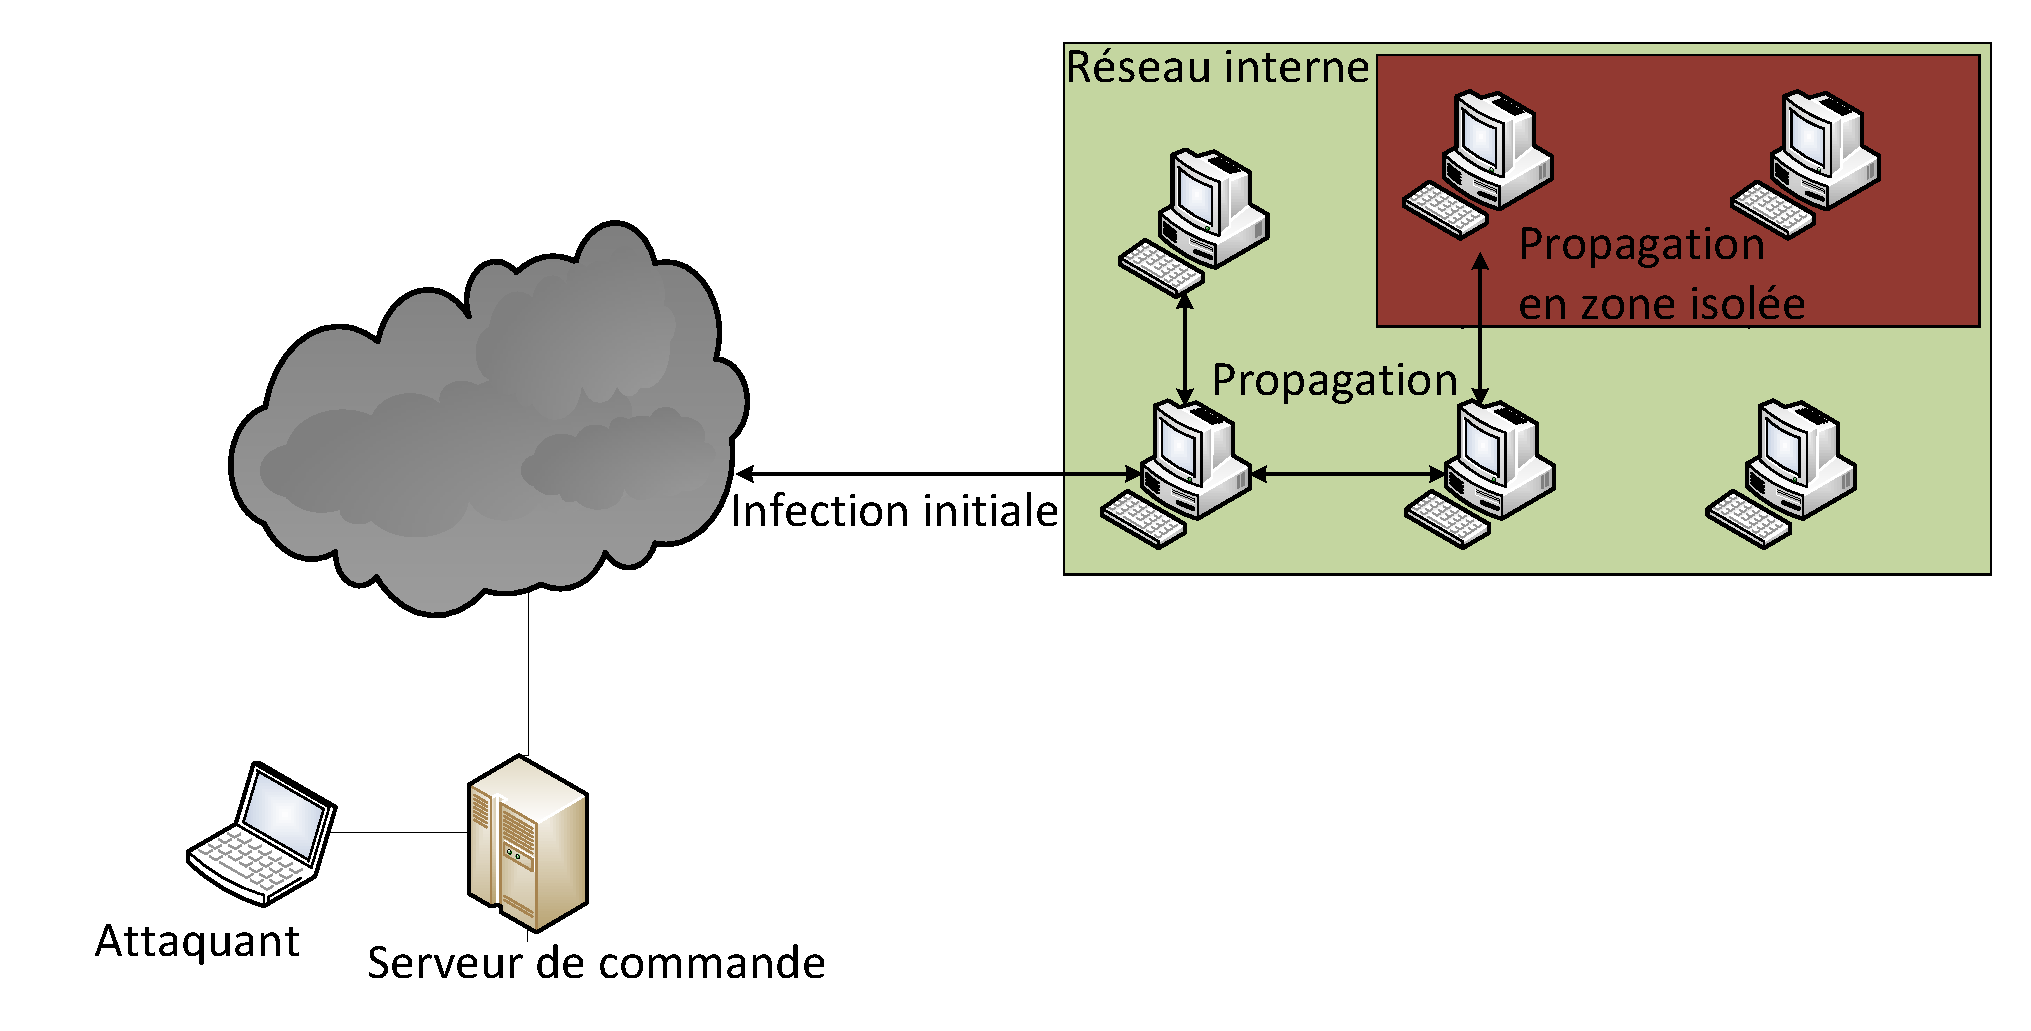
\includegraphics[width=0.8\textwidth]{AThierry/img/propagationDuqu.pdf}
 % graph11.eps: 0x0 pixel, 300dpi, 0.00x0.00 cm, bb=0 0 384 336
\end{center}
\caption{Schéma de propagation en profondeur de Duqu}
\label{fig:AThierry_propagationDuqu}
\end{figure}


\section{Reconstruction du code du driver}
Nous savions que \Duqu\ partage du code avec Stuxnet puisque nous avons exhibé des parties équivalentes dans les DLL principales de chacun des malware \cite{AThierry_REAT12} et Symantec a détaillé des similarités dans la technique d'injection de la DLL et dans certaines ressources (exports et routines).
Pourquoi alors s'intéresser au driver de \Duqu\ alors que celui de \Stuxnet, similaire, a été décompilé par Amr Thabet \cite{AThierry_ThabetDriver} ?
En réalité le diable est dans les détails car l'analyse détaillée d'une souche du driver découverte en octobre 2011 en Europe (\driver) a montré de nombreuses singularités par rapport à \Stuxnet\ dans sa méthode d'injection et ses mécanismes de furtivité.

Nous avons donc travaillé sur la rétroingénierie de cette version spécifique du driver afin d'en documenter les fonctionnalités.
Notre objectif est d'obtenir un code compréhensible, qui compile, et dont la version compilée soit au plus proche du driver original.


\subsection{Décompilation avec IDA}
Nous avons utilisé le module de décompilation "Hex-Rays Decompiler", intégré à IDA sous la forme d'un plugin \cite{AThierry_IDADecompiler}. Il permet de générer un pseudo-code C à partir du fichier binaire en cours d'analyse. Il produit non seulement du code source mais facilite également sa réécriture directement à l'intérieur de l'interface graphique du plugin. % (menu {\em Open subviews Pseudocode F5}).
Malheureusement le code en sortie n'est, dans notre cas, pas exploitable directement. D'une part le code n'est pas compilable parce que des types de variables n'ont pas été correctement reconnus et certaines conventions d'appel ne sont pas standard (non reconnues par le décompilateur). De plus le code généré est difficilement lisible, en partie parce que certaines structures n'ont pas été identifiées. Nous détaillerons dans les paragraphes suivants ces difficultés et des moyens de résolution.

Nous avons procédé de manière incrémentale afin de reconstruire le code petit à petit en vérifiant à chaque étape que le code compile et qu'une fois compilé il est équivalent à celui du binaire \driver\ original. 
Cela a consisté à :
\begin{itemize}
 \item Commenter tout le pseudo-code sauf la fonction du point d'entrée du driver (\emph{DriverEntry}) et les variables globales s'y rapportant
 \item Régler chaque erreur une par une
 \item Comparer le code compilé au binaire original, modifier le code pour s'en rapprocher
 \item Ajouter du code auparavant commenté et revenir à l'étape de correction d'erreurs.
\end{itemize}

\begin{figure}
\begin{changemargin}{-0cm}{-0cm}
\includegraphics[width=1.0\textwidth]{AThierry/img/decompil.pdf}
\end{changemargin}
\caption{À gauche, le code source initialement généré par IDA. À droite, une fois le type de la variable \texttt{BaseAddress} re-défini.}
\label{fig:AThierry_decompil}
\end{figure}

\subsection{Identification des structures et des types}
Comme on peut s'en rendre compte sur la partie gauche de la figure \ref{fig:AThierry_decompil}, le décompilateur n'arrive pas toujours à déterminer le type d'une variable.
On prend l'exemple de la fonction \texttt{ParsePE}, utilisée pour chercher des informations dans les binaires chargés en mémoire.
On part donc à la pêche aux indices : ici le test sur la valeur magique "\texttt{MZ}" nous laisse à penser que la fonction porte sur un traitement de l'entête d'un fichier exécutable au format PE, ce qui nous permet d'en déduire que la variable \texttt{BaseAddress} est un pointeur sur une structure \texttt{IMAGE\_DOS\_HEADER}. Une fois le type de la variable correctement défini, IDA identifie automatiquement le nom du champ de la structure à l'{\em offset} indiqué nous épargnant de longues recherches dans la documentation de Microsoft (par exemple l'{\em offset} 60 soit 0x3C en hexadécimal correspond au champ \texttt{e\_lFanew} de la structure \texttt{IMAGE\_DOS\_HEADER}). Si la structure est propre au programme analysé, nous pouvons la définir à travers le plugin de décompilation après une analyse manuelle.

% \begin{figure}
% %\begin{changemargin}{-2cm}{-2cm}
% \includegraphics[width=1.0\textwidth]{AThierry/img/pseudocode-final.pdf}
% %\end{changemargin}
% \caption{Modification du code source depuis le plugin d'IDA}
% \label{fig:pseudocodefinal}
% \end{figure}

Au final, nous avons retouché le code pour obtenir un code compréhensible pour un développeur C (figure \ref{fig:AThierry_ParsePEFunction}).
Ce n'est pas encore un code ``propre'' : par exemple un développeur n'aurait pas utilisé de \emph{goto} pour gérer un traitement commun à la fin d'une condition mais l'aurait plutôt placé après la disjonction des cas, et il aurait rajouté une clause \emph{else} pour le cas par défaut. Après cette réorganisation, les objectifs sont atteints : pour la fonction \texttt{ParsePE}, le code (re)compilé est proche du binaire original, et le code source reconstruit est exploitable.

La lisibilité du code ainsi obtenu nous permet de détecter une erreur de programmation comme à la deuxième ligne ici :

 \begin{center}
 \begin{changemargin}{-1cm}{-1cm}
\begin{lstlisting}[language={C}]
  else if ((pFileHeader->Machine ^ 0xDE67) == (IMAGE_PE_x86_MACHINE ^ 0xDE67) 
           && (pOptionHeader->Magic ^ 0x5A08) == IMAGE_PE32_PLUS_MAGIC 
           && pFileHeader->SizeOfOptionalHeader == 0xF0 ) // 0x5803 64bits
\end{lstlisting}
\hspace{1cm} Au lieu de :
\begin{lstlisting}[language={C}]
  else if ((pFileHeader->Machine ^ 0xDE67) == (IMAGE_PE_x86_MACHINE ^ 0xDE67) 
           && (pOptionHeader->Magic ^ 0x5A08) == (IMAGE_PE32_PLUS_MAGIC ^ 0x5A08) 
           && pFileHeader->SizeOfOptionalHeader == 0xF0 ) // 0x5803 64bits
\end{lstlisting}
 \end{changemargin}
 \end{center}

Le test mis en place omet un XOR sur la constante IMAGE\_PE32\_PLUS\_MAGIC. Ce test devrait permettre de reconnaître un binaire 64 bits et de définir une table d'import en conséquence. Avec cette erreur, \Duqu\ est incapable de parser un binaire 64 bits (un code d'erreur est renvoyé). De fait cette version du driver ne fonctionne pas sur un Windows 64 bits.

\begin{figure}
\begin{changemargin}{-1cm}{-1cm}
\scriptsize
\begin{lstlisting}[language={C}]
NTSTATUS __cdecl ParsePE(
      __out PEDataPtr pPEData, 
      __in PIMAGE_DOS_HEADER BaseAddress,
      __in int flag)
{
  PVOID infosPE; //IMAGE_NT_HEADER; 
  PIMAGE_DOS_HEADER  pDosHeader     = NULL;
  PIMAGE_NT_HEADERS  pNtHeader      = NULL;
  PIMAGE_FILE_HEADER  pFileHeader   = NULL;
  PIMAGE_OPTIONAL_HEADER32  pOptionHeader = NULL;
  PVOID pExportTableRVA; 

  infosPE=(PIMAGE_DOS_HEADER)BaseAddress; 
  if (((PIMAGE_DOS_HEADER)infosPE)->e_magic != 'ZM' )
    return STATUS_WAIT_1;

  pNtHeader = (PIMAGE_NT_HEADERS32)((DWORD)infosPE + ((PIMAGE_DOS_HEADER)infosPE)->e_lfanew);
  // hash of 'P' 'E' '0' '0' (0x00004550) => 0x0F750B7D4
  if ( (pNtHeader->Signature ^ 0xF750F284) != (IMAGE_NT_SIGNATURE ^ 0xF750F284)) 
    return STATUS_WAIT_1; 

  pFileHeader = (PIMAGE_FILE_HEADER)&pNtHeader->FileHeader;
  pOptionHeader = (PIMAGE_OPTIONAL_HEADER32)&((PIMAGE_NT_HEADERS32)infosPE)->OptionalHeader;
  if ((pFileHeader->Machine ^ 0x594F) == (IMAGE_PE_i386_MACHINE ^ 0x594F)) 
  {
    if ((pOptionHeader->Magic ^ 0x5908) == (IMAGE_PE32_MAGIC ^ 0x5908) && (pFileHeader->SizeOfOptionalHeader == 0xE0 ))  
    {
      pPEData->Status = 0;
      pExportTableRVA = (PVOID)&(pOptionHeader->DataDirectory[IMAGE_DIRECTORY_ENTRY_EXPORT]).VirtualAddress;  

Continue:
      pPEData->ExportTableRVA=pExportTableRVA;     
      pPEData->dwSizeOfImage = pOptionHeader->SizeOfImage;  
      pPEData->lpDataDir=pFileHeader->SizeOfOptionalHeader + (BYTE *)&(pFileHeader->Characteristics) + sizeof(WORD);                                                              
      pPEData->ResourceDataDir=(ULONG)infosPE;                        
      pPEData->PEAddress1=pPEData->PEAddress2;                        
      pPEData->wNumberOfSections=pFileHeader->NumberOfSections;       
      pPEData->PEAddress2=(PIMAGE_DOS_HEADER)&((PIMAGE_NT_HEADERS32)infosPE)->Signature; 
      return STATUS_SUCCESS;
     }
  }
  else if ((pFileHeader->Machine ^ 0xDE67) == (IMAGE_PE_x86_MACHINE ^ 0xDE67) 
           && (pOptionHeader->Magic ^ 0x5A08) == IMAGE_PE32_PLUS_MAGIC 
           && pFileHeader->SizeOfOptionalHeader == 0xF0 ) // 0x5803 64bits
  {
    pPEData->Status = 1;
    pExportTableRVA = (PVOID)&(pOptionHeader->DataDirectory[IMAGE_DIRECTORY_ENTRY_RESOURCE]).VirtualAddress; 
    goto Continue;
  }
  return STATUS_WAIT_1;
}
\end{lstlisting}
\caption{Code source final de la fonction ParsePE\label{fig:AThierry_ParsePEFunction}}
\end{changemargin}
\end{figure}

% \clearpage
\subsection{Conventions d'appel}

Pour chaque routine, IDA cherche à déterminer la convention d'appel utilisée à partir des registres qui sont lus avant d'être écrits (paramêtres) et ceux écrits sans être lus après (valeur de retour). Si ces registres correspondent à un appel classique, il l'annote dans le code C pour que le compilateur respecte la convention. Les conventions d'appel de Microsoft Visual C++ sont données Figure \ref{fig:AThierry_callingconvention}, l'appel par défaut étant \emph{thiscall}. Dans le cas où il ne détermine pas la convention, il annote les registres d'entrée et de sortie en notant qu'il s'agit d'un appel non conventionnel (\emph{usercall}) et met la définition de la fonction en commentaire (ici les arguments sont passés dans les registres \texttt{edi} et \texttt{esi}) :
\begin{changemargin}{-0.4cm}{-0.4cm}
\begin{lstlisting}[language={C}, escapechar=!]
!//! int __usercall SearchForCodeInSystem<eax>(int *a1<edi>, int a2<esi>);
\end{lstlisting}
\end{changemargin}

Une convention d'appel non standard est détectée dans le cas où une partie de la fonction a été écrite directement en assembleur ou à la suite d'une optimisation faite par le compilateur. On doit alors réécrire la fonction à la main (en partie en assembleur) ou choisir à la main une convention d'appel.

\begin{figure}
\begin{center}
\begin{tabular}{|l|c|c|c|c|}
\hline 
Convention & Arguments & \emph{this} (C++) & Retour & Nettoie la pile\\
\hline
C (\_\_cdelcl) & pile & (argument) & eax & appelant\\
Standard (\_\_stdcall) & pile & (argument) & eax & appelé\\
Thiscall (\_\_thiscall) & pile & ecx & eax & appelé\\
Fastcall (\_\_fastcall) & ecx, edx, pile & (argument) & eax & appelé\\
\hline
\end{tabular}
\end{center}
\caption{Conventions d'appel dans leur version Visual C++}
\label{fig:AThierry_callingconvention}
\end{figure}

\section{Analyse fonctionnelle du driver à partir de son code source}

Une fois le code du driver reconstitué, décrivons en détail son fonctionnement.
Il y a deux phases principales, la première consiste en la mise en place du driver : il demande au système d'être notifié en cas de chargement de binaires et initialise ses mécanismes de furtivité.
La seconde phase est lancée lorsque des notifications sont signalées chargeant un binaire cible. Le driver infecte alors le binaire en y injectant la DLL de \Duqu\ puis celle-ci active la charge finale.

\subsection{Initialisation du driver lors du démarrage du système}
La séquence de démarrage des drivers système sous Windows est déterminée par le positionnement de la clé de registre \texttt{Group}. Ainsi en fonction de son groupe d'appartenance (\driver\ fait partie du groupe "network"), le driver sera démarré plus ou moins tôt lors de la séquence de boot. Le système d'exploitation donne automatiquement la main aux drivers prioritaires avant même que la couche d'abstraction matérielle (HAL) ne soit chargée en mémoire. 

Le driver, une fois démarré, commence par allouer un emplacement mémoire de 512 octets destiné à contenir un tableau de pointeurs de fonctions partagées entre les différentes routines de "callback". A la suite de cela, il passe au déchiffrement de ses paramètres internes (avec la fonction donnée en figure \ref{fig:AThierry_decrypt}) nous révélant ainsi le nom et l'emplacement de la clé de registre utilisée pour la configuration de "l'injection" mais également le nom sous lequel le driver va s'enregistrer au près du gestionnaire.  
\begin{figure}
\scriptsize
\begin{changemargin}{-1cm}{-1cm}
\begin{lstlisting}[language={C}]
 void __fastcall decode_parameters(
      __in PUNICODE_STRING RegistryPath)
{
  ULONG dwSeed; 
  UINT32 dwCount; 

  dwSeed = 0x7EF640F0;
  dwCount = 0;
  
  do
  {
    g_DefaultParamCrypted[dwCount++] ^= (char) dwSeed;
    dwSeed = ((((dwSeed & 0xFFFFFFFB) << 28) | (dwSeed >> 5)) * (((dwSeed & 0xFFFFFFFB) << 28) 
    | (dwSeed >> 5)) / 0x8677 + 0x787C956A * (((dwSeed & 0xFFFFFFFB) << 28) | (dwSeed >> 5)) + 1) 
    ^ (((dwSeed & 0xFFFFFFFB) << 28) | (dwSeed >> 5));
  } while (dwCount < 428 );

  if ( (char)g_LocalParameters == 0) { 
      //Recopie le chemin de la cle de registre lorsque cela est necessaire
      memcpy((void *)&g_LocalParameters, RegistryPath->Buffer, RegistryPath->Length);
  }
}
\end{lstlisting}
\end{changemargin}
\caption{Routine de déchiffrement utilisée pour les paramètres internes (également utilisée sur la DLL à injecter).}
\label{fig:AThierry_decrypt}
\end{figure}



Si le déchiffrement s'est correctement déroulé, vient alors la vérification du mode d'exécution : soit le système s'avère être en mode sans échec ou en mode débogage, dans ce cas le driver termine son exécution ; soit en mode normal alors il commence par créer un device répondant au doux nom de $\backslash$\texttt{Device}$\backslash$\texttt{\{624409B3-4CEF-41c0-8B81-7634279A41E5\}} puis il définit la liste des commandes de contrôle qu'il sera à même de traiter (une grande majorité des commandes commencent par  \texttt{IRP\_MJ\_} tels que \texttt{IRP\_MJ\_CREATE}, \texttt{IRP\_MJ\_READ}, etc.).

Ceci étant fait, il enregistre auprès du gestionnaire d'événements interne du noyau, deux fonctions de rappel ({\em callback function}). La première est nécessaire au gestionnaire du \texttt{Plug and Play} (\texttt{PnP}). On y trouve des opérations classiques pour un driver, à savoir la création d'un point d'accès sur celui-ci ($\backslash$\texttt{Device}$\backslash$\texttt{Gpd0}), ainsi qu'un lien ($\backslash$\texttt{DosDevices}$\backslash$\texttt{GpdDev}) et enfin l'attachement de l'objet \texttt{Device} à une pile mémoire. Quant à la seconde, elle sera exécutée lorsque le driver devra être initialisé ou réinitialisé (à la différence de la première, cette fonction est insérée dans une liste d'attente d'événements et supprimée à l'issue de son traitement). 
  
Cette seconde fonction embarque un mécanisme d'attente de fin de chargement du noyau Windows. Pour cela, une fonction vérifie qu'il est possible d'accéder à la DLL \texttt{hal.dll}. Si tel n'est pas le cas, la fonction de réinitialisation est de nouveau insérée dans la file d'attente des traitements pour un maximum de 200 fois. 
Lors de la fin de chargement du système, un point d'accès $\backslash$\texttt{Device}$\backslash$\texttt{Gpd1} est alors créé puis une routine de traitement des requêtes lui est associé. À ce stade le driver est à même de dialoguer avec une application s'exécutant en mode utilisateur (ring 3). 

La mise en place des fonctions du rootkit va pouvoir débuter. On parle ici de rootkit car ce dispositif ne peut pas se permettre d'utiliser des appels systèmes réputés pour être couramment employées par les malwares et donc particulièrement surveillées par les antivirus. En particulier les fonctions d'allocation d'espace mémoire dans d'autres processus (tels \texttt{VirtualAllocEx} et \texttt{ZwAllocateVirtualMemory}), car elles permettent d'injecter du code dans un processus cible. Mais pour accomplir sa tâche, qui va consister à déposer un \emph{HOOK} sur le point d'entrée d'une application système, \Duqu\ a également besoin de faire appel à la fonction \texttt{ZwProtectVirtualMemory} que Microsoft a délibérément omise de la liste des fonctions accessibles en dehors du kernel. C'est pourquoi la stratégie de \Duqu\ va consister à retrouver cette fonction en mémoire afin de réaliser des appels directs sans passer par le système standard des imports.

Ainsi le driver part à la recherche des fonctions \texttt{ZwAllocateVirtualMemory} et \texttt{ZwProtectVirtualMemory} afin de localiser leur emplacement mémoire tout en se préservant d'éventuelles détections. Le procédé que nous allons voir ensemble est remarquable d'ingéniosité car ces deux fonctions sont implémentées directement au c\oe ur du noyau système (fichier \texttt{Ntoskrnl.exe} ou \texttt{ntkrnlpa.exe} suivant la version de l'OS). 

Une première fonction se charge de passer en revue la liste de tous les modules chargés par le système de démarrage (DLLs et exécutables) jusqu’à identifier l'un des deux fichiers recherchés en comparant leurs noms. Cette liste est obtenue à l'aide de la fonction système \texttt{ZwQuerySystemInformation}. 

Lorsque le fichier noyau est déniché, le processus prend connaissance de son emplacement mémoire afin de le soumettre à une seconde fonction qui va le disséquer. 

Le fichier noyau est au format \texttt{PE} (\texttt{Portable Executable}). Sur la figure \ref{fig:AThierry_ParsePEFunction} précédemment évoquée, nous pouvons voir comment cette fonction procède pour s'assurer qu'il s'agit bien d'un fichier exécutable et pour déterminer l'emplacement des sections et de la table d'export. Elle réalise un contrôle sur les valeurs remarquables telles que '\texttt{MZ}', '\texttt{IMAGE\_NT\_SIGNATURE}', '\texttt{IMAGE\_PE\_i386\_MACHINE}, '\texttt{IMAGE\_PE\_x86\_MACHINE}', '\texttt{IMAGE\_PE32\_MAGIC}' ou encore '\texttt{IMAGE\_PE32\_PLUS\_MAGIC}' et progresse dans le fichier jusqu'à atteindre la partie définissant les sections. Ces constantes sont bien entendu obfusquées (avec un {\em XOR}) afin de ne pas éveiller de soupçons.

Une fois arrivée aux sections, la fonction va rechercher celle contenant le code exécutable des fonctions systèmes (section nommée \texttt{.text} ou \texttt{PAGE} et de type \texttt{IMAGE\_SCN\_MEM\_EXECUTE}, \texttt{IMAGE\_SCN\_MEM\_READ}, \texttt{IMAGE\_SCN\_CNT\_CODE}). Là encore, dans un esprit de furtivité, elle utilise une fonction de hachage sur le nom des sections rencontrées et compare le nom haché à la valeur désirée (voir la figure \ref{fig:AThierry_kernel}). 
\begin{figure}
% \scriptsize
%         if ( pPEDataPtr->wNumberOfSections > 0 )
%         {
%           NumberOfSections = pPEDataPtr->wNumberOfSections;
%           OrdinalValue[1] = 0;
%           while ( 1 )
%           {
% ...
%             }
%             ++wIndex;
%             if ( wIndex >= NumberOfSections )
%             {
%               if ( !*(ULONG *)&OrdinalValue[1] )
%                 break;
%               g_ZwProtectVirtualMemoryADDR  = *(ULONG *)&OrdinalValue[1];   
%               goto LABEL_15;
%             
%           } 
%         }
%       }
%       goto LABEL_15bis;
%     }
%   }
%   return result;
% }
% \begin{framed}
\begin{changemargin}{-1cm}{-1cm}
\begin{lstlisting}[language={C}]
pSectionHeader=(PIMAGE_SECTION_HEADER)(pFirstSectionHeader+sizeof(IMAGE_SECTION_HEADER)*wIndex);
if ( ((ULONG)(((PIMAGE_SECTION_HEADER)((DWORD)pPEDataPtr->lpDataDir+sizeof(IMAGE_SECTION_HEADER) 
      * wIndex))->Characteristics) & (IMAGE_SCN_MEM_EXECUTE| IMAGE_SCN_MEM_READ 
      | IMAGE_SCN_MEM_DISCARDABLE | IMAGE_SCN_CNT_CODE)) == (IMAGE_SCN_MEM_EXECUTE
      | IMAGE_SCN_MEM_READ | IMAGE_SCN_CNT_CODE) )  
{
  SecNameHash = HashOfSectionName((BYTE *)((DWORD)pPEDataPtr->lpDataDir
		+ sizeof(IMAGE_SECTION_HEADER) * wIndex));

  if ( SecNameHash == 0x4B93B9A8 || SecNameHash == 0x1294971C ) // hachage de ".text" et "PAGE"
  {
    SectionPhysicalAddress = (ULONG)(pSectionHeader->SizeOfRawData);
    if ( (ULONG)(pSectionHeader->Misc.PhysicalAddress) < SectionPhysicalAddress )
	SectionPhysicalAddress = (ULONG)(pSectionHeader->Misc.PhysicalAddress);
    OrdinalValue[0] = 1;                                                            
    FindCode(pPEDataPtr, pBaseAddress + pSectionHeader->VirtualAddress, pBaseAddress 
	      + SectionPhysicalAddress + pSectionHeader->VirtualAddress, &OrdinalValue[1], 
	      (BYTE *)&Status);
    if ( OrdinalValue[0] )
      break;
  }
}
\end{lstlisting}
\end{changemargin}
% \end{framed}
\caption{Extrait de la routine de traitement du noyau système.\label{fig:AThierry_kernel}}
\end{figure}

Maintenant que la section a été débusquée, une nouvelle fonction va se charger de localiser une fonction système faisant appel à \texttt{ZwProtectVirtualMemory} sous la forme d'un \texttt{call} (voir la figure \ref{fig:AThierry_CallZwProtect}), étape nécessaire car cette fonction n'est pas exportée par le noyau.

\begin{figure}
\scriptsize
% \begin{framed}
% PAGE:004ED1AD                      loc_4ED1AD:                             
% PAGE:004ED1AD 6A 04                push    4               ; Protect
% PAGE:004ED1AF 68 00 10 00 00       push    1000h           ; AllocationType
% PAGE:004ED1B4 8D 45 10             lea     eax, [ebp+arg_8]
% PAGE:004ED1B7 50                   push    eax             ; AllocationSize
% PAGE:004ED1B8 53                   push    ebx             ; ZeroBits
% PAGE:004ED1B9 8D 45 FC             lea     eax, [ebp+BaseAddress]
% PAGE:004ED1BC 50                   push    eax             ; BaseAddress
% PAGE:004ED1BD 57                   push    edi             ; ProcessHandle
% PAGE:004ED1BE E8 19 8C F1 FF       call    ZwAllocateVirtualMemory
% PAGE:004ED1C3 3B C3                cmp     eax, ebx
% PAGE:004ED1C5 8B 4D FC             mov     ecx, [ebp+BaseAddress]
% PAGE:004ED1C8 89 4E 0C             mov     [esi+0Ch], ecx
% PAGE:004ED1CB 7C 2E                jl      short loc_4ED1FB
% PAGE:004ED1CD 38 5D 0B             cmp     byte ptr [ebp+ProcessHandle+3], bl
% PAGE:004ED1D0 74 27                jz      short loc_4ED1F9
% PAGE:004ED1D2 8B 45 D0             mov     eax, [ebp+var_30]
% PAGE:004ED1D5 89 45 F8             mov     [ebp+ProtectSize], eax
% PAGE:004ED1D8 8D 45 F4             lea     eax, [ebp+OldProtect]
% PAGE:004ED1DB 50                   push    eax             ; OldProtect
% PAGE:004ED1DC 68 04 01 00 00       push    104h            ; NewProtect
% PAGE:004ED1E1 8D 45 F8             lea     eax, [ebp+ProtectSize]
% PAGE:004ED1E4 50                   push    eax             ; ProtectSize
% PAGE:004ED1E5 8D 45 FC             lea     eax, [ebp+BaseAddress]
% PAGE:004ED1E8 50                   push    eax             ; BaseAddress
% PAGE:004ED1E9 57                   push    edi             ; ProcessHandle
% PAGE:004ED1EA E8 93 96 F1 FF       call    ZwProtectVirtualMemory
% PAGE:004ED1EF 3B C3                cmp     eax, ebx
% PAGE:004ED1F1 7C 08                jl      short loc_4ED1FB
% PAGE:004ED1F3 8B 45 F8             mov     eax, [ebp+ProtectSize]
% PAGE:004ED1F6 01 46 0C             add     [esi+0Ch], eax
\begin{changemargin}{-0.5cm}{-0.5cm}
\begin{lstlisting}[language={[x86masm]Assembler}, escapechar=!]
PAGE:004ED1AD                  loc_4ED1AD: [...]                      
PAGE:004ED1BC 50               push    eax             ; BaseAddress
PAGE:004ED1BD 57               push    edi             ; ProcessHandle
PAGE:004ED1BE E8 19 8C F1 FF   call    ZwAllocateVirtualMemory
PAGE:004ED1C3 3B C3            cmp     eax, ebx
PAGE:004ED1C5 8B 4D FC         mov     ecx, [ebp+BaseAddress]
PAGE:004ED1C8 89 4E 0C         mov     [esi+0Ch], ecx
PAGE:004ED1CB 7C 2E            jl      short loc_4ED1FB
PAGE:004ED1CD 38 5D 0B         cmp     byte ptr [ebp+ProcessHandle+3], bl
PAGE:004ED1D0 74 27            jz      short loc_4ED1F9
PAGE:004ED1D2 8B 45 D0         mov     eax, [ebp+var_30]
PAGE:004ED1D5 89 45 F8         mov     [ebp+ProtectSize], eax
PAGE:004ED1D8 8D 45 F4         lea     eax, [ebp+OldProtect]
PAGE:004ED1DB 50               push    eax             ; OldProtect
PAGE:004ED1DC 68 04 01 00 00   push    104h            ; NewProtect
PAGE:004ED1E1 8D 45 F8         lea     eax, [ebp+ProtectSize]
PAGE:004ED1E4 50               push    eax             ; ProtectSize
PAGE:004ED1E5 8D 45 FC         lea     eax, [ebp+BaseAddress]
PAGE:004ED1E8 50               push    eax             ; BaseAddress
PAGE:004ED1E9 57               push    edi             ; ProcessHandle
PAGE:004ED1EA E8 93 96 F1 FF   call    ZwProtectVirtualMemory
PAGE:004ED1EF 3B C3            cmp     eax, ebx
\end{lstlisting}
\end{changemargin}
% \end{framed}
\caption{Fonction faisant appel à \texttt{ZwProtectVirtualMemory}.\label{fig:AThierry_CallZwProtect}}
\end{figure}

La fonction recherchée contient l'opcode \texttt{push 104h} (encodé en \texttt{68 04 01 00 00}) et réalise un \texttt{call} (encodé en \texttt{E8}) un peu plus loin dans le code.
Sachant que cette fonction effectue au préalable un appel vers la fonction \texttt{ZwAllocateVirtualMemory}, la recherche remonte jusqu'à trouver cet appel (l'adresse du \texttt{call} est comparée à celle de la fonction \texttt{ZwAllocateVirtualMemory} exportée par le noyau), puis redescend au prochain \texttt{call} (à l'adresse \texttt{0x004ED1EA}) qui est l'appel vers \texttt{ZwProtectVirtualMemory} recherché.

Le processus vérifie dans un premier temps que l'adresse trouvée pour la fonction \texttt{ZwProtectVirtualMemory} est bien située dans une fonction du noyau pour s'assurer qu'elle n'est pas déroutée vers une fonction de surveillance.
Dans un second temps, elle contrôle son intégrité par l'application d'un masque sur les 32 octets composant la routine avec un \texttt{AND} logique (voir figure \ref{fig:AThierry_matching}). Ces vérifications sont également effectuées pour la fonction \texttt{ZwAllocateVirtualMemory}.

% \begin{figure}
% \scriptsize
% % \begin{framed}
% \begin{changemargin}{-1cm}{-1cm}
% \begin{lstlisting}[language={[x86masm]Assembler}]
% .text:0044A0EE                 add     esi, eax
% .text:0044A0F0                 mov     [ebp+BaseAddress], esi
% .text:0044A0F3                 push    4               ; Protect
% .text:0044A0F5                 push    eax             ; AllocationType
% .text:0044A0F6                 lea     eax, [ebp+AllocationSize]
% .text:0044A0F9                 push    eax             ; AllocationSize
% .text:0044A0FA                 push    ebx             ; ZeroBits
% .text:0044A0FB                 lea     eax, [ebp+BaseAddress]
% .text:0044A0FE                 push    eax             ; BaseAddress
% .text:0044A0FF                 push    0FFFFFFFFh      ; ProcessHandle
% .text:0044A101                 call    ZwAllocateVirtualMemory
% .text:0044A106                 mov     [ebp+var_28], eax
% .text:0044A109                 cmp     eax, ebx
% .text:0044A10B                 jl      short loc_44A140
% .text:0044A10D                 mov     eax, [ebp+BaseAddress]
% .text:0044A110                 mov     [edi], eax
% .text:0044A112                 jmp     short loc_44A140
% .text:0044A114 ; -----------------------------------------------------------
% .text:0044A114
% .text:0044A114 loc_44A114:                             
% .text:0044A114                 add     ecx, 1000h
% .text:0044A11A                 mov     [edi], ecx
% .text:0044A11C                 push    104h            ; Protect
% .text:0044A121                 push    eax             ; AllocationType
% .text:0044A122                 lea     eax, [ebp+AllocationSize]
% .text:0044A125                 push    eax             ; AllocationSize
% .text:0044A126                 push    ebx             ; ZeroBits
% .text:0044A127                 lea     eax, [ebp+BaseAddress]
% .text:0044A12A                 push    eax             ; BaseAddress
% .text:0044A12B                 push    0FFFFFFFFh      ; ProcessHandle
% .text:0044A12D                 call    ZwAllocateVirtualMemory
% .text:0044A132                 mov     [ebp+var_28], eax
% \end{lstlisting}
% \end{changemargin}
% % \end{framed}
% \caption{Fonction faisant appel à ZwAllocateVirtualMemory.\label{fig:CallZwAlloc}}
% \end{figure}


\begin{figure}
\begin{center}
 \includegraphics[width=1.0\textwidth]{AThierry/img/mask.pdf}
\end{center}
\caption{Application du masque d'intégrité sur les fonctions \texttt{ZwAllocateVirtualMemory} et \texttt{ZwProtectVirtualMemory}. Les valeurs qui doivent être identiques sont en gris clair.}
\label{fig:AThierry_matching}
\end{figure}

% Lorsque le driver est exécuté sur un système Windows 2000, la technique employée diffère. Cette fois-ci une fonction va parcourir le code à la recherche non pas de l'opcode \texttt{push 104h} mais de \texttt{mov eax, 77h} (encodé en \texttt{B8 77 00 00 00}) afin de localiser directement la routine \texttt{ZwProtectVirtualMemory} (voir la figure \ref{fig:ZwProtectVirtualMemory}) puis de vérifier que chaque opcode est semblable à celui contenu dans le code du driver. 

% \begin{figure}
% % \begin{framed}
% \scriptsize
% \begin{changemargin}{-1cm}{-1cm}
% \begin{lstlisting}[language={[x86masm]Assembler}]
% .text:00400F2A B8 77 00 00 00  mov   eax, 77h
% .text:00400F2F 8D 54 24 04     lea   edx, [esp+ProcessHandle]
% .text:00400F33 CD 2E           int   2Eh    ; DOS 2+ internal - EXECUTE COMMAND
% .text:00400F33                ; DS:SI -> counted CR-terminated command string
% .text:00400F35 C2 14 00        retn  14h
% \end{lstlisting}
% \end{changemargin}
% % \end{framed}
% \caption{Appel système de la fonction \texttt{ZwProtectVirtualMemory} sous Windows 2000.\label{fig:ZwProtectVirtualMemory}}
% \end{figure}

A présent, l'adresse de la fonction \texttt{ZwProtectVirtualMemory} peut être mémorisée pour une future utilisation discrète. 

Vient alors l'initialisation d'un espace mémoire partagé servant de lien entre les différentes fonctions de rappel au sein du noyau (ring 0). Il va servir à stocker, entre autres, les paramètres d'infection extraits depuis la base de registre une fois déchiffrés, mais également une structure (voir la figure \ref{fig:AThierry_InjectedDataStruct}) donnant accès à des fonctions système situées dans la DLL Kernel32.dll. Enfin, pour ses besoins interne, il va constituer une table d'import donnant accès à des fonctions situées au c\oe ur du noyau (voir la figure \ref{fig:AThierry_NtoskrnlIAT}). Cette table d'import pourra être utilisée par la suite par les différents codes injectés ainsi que la charge finale.
\begin{figure}
% \begin{framed}
\scriptsize
\begin{changemargin}{-1cm}{-1cm}
\begin{lstlisting}[language={C}]
typedef struct _INJECTEDDATA  
{ 
LONGLONG Kernel32Imagebase;      // Adresse de base de kernel32.dll
LONGLONG VirtualAlloc;           // Pointeurs sur les fonctions de Kernel32 utilisees par le code injecte
LONGLONG VirtualFree;           
LONGLONG GetProcAddress;   
LONGLONG GetModuleHandleA; 
LONGLONG LoadLibraryA;      
LONGLONG LoadLibraryW;     
LONGLONG lstrcmpA;         
LONGLONG lstrcmpiA;        
LONGLONG GetVersionExA;    
LONGLONG DeviceIoControl;  
LONGLONG InjectedSupModuleStart;  // Pointeur sur le debut de la memoire allouee dans le processus cible
LONGLONG InjectedSupModuleMZoffset; // Offset du debut du code tremplin injecte
LONGLONG InjectedSupModuleSize;  // Taille du code tremplin injecte
LONGLONG InjectedDLLImagebase;   // Pointeur sur le debut de la DLL injectee             
ULONG EntryPoint1stDword;        // Sauvegarde des douze premiers octets du point d'entree de la cible
ULONG EntryPoint2snDword;  
ULONG EntryPoint3rdDword;  
ULONG Reserved15;                   
ULONG OldMemProtect;             // Sauvegarde des droits d'acces originaux
ULONG Reserved17;                   
HANDLE handle;                   // Sauvegarde de l'Handle permettant de communiquer avec le driver depuis l'espace utilisateur
ULONG Reserved18;                
}_INJECTEDDATA, *PINJECTEDDATA;
\end{lstlisting}
\end{changemargin}
% \end{framed}
\caption{Structure mémorisée dans un espace mémoire partagé.\label{fig:AThierry_InjectedDataStruct}}
\end{figure}
  
\begin{figure}
% \begin{framed}
\scriptsize
%   g_RtlGetVersionADDR = 0;
%   g_KeAreAllApcsDisabledADDR = 0;
%   g_PsGetProcessSessionIdADDR = 0;
%   g_PsGetProcessPebADDR = 0;
%   g_PsSetLoadImageNotifyRoutineADDR = 0;
%   g_ZwAllocateVirtualMemoryADDR = 0;
%   g_KeStackAttachProcessADDR = 0;
%   g_KeUnstackDetachProcessADDR = 0;
\begin{changemargin}{-1cm}{-1cm}
\begin{lstlisting}[language={C}]
int *__cdecl InitializeIAT()
{
  PIMAGE_DOS_HEADER pBaseAddress; 
  int KeUnstackDetachProcessTmp; 
  struct _PEData pedata;
  PEDataPtr pPEData=NULL; 

  pBaseAddress = SearchNtoskrnl();

  if ( pBaseAddress )
  {
    if ( !ParsePE((PEDataPtr)&pPEData, pBaseAddress,1) )
    {
      // Recherche de la fonction PsSetLoadImageNotifyRoutine()
      g_PsSetLoadImageNotifyRoutineADDR = GetApiFromKernel32((PEDataPtr)&pPEData, 0x0AA67394D); 
      // Recherche de la fonction ZwAllocateVirtualMemory()
      g_ZwAllocateVirtualMemoryADDR     = GetApiFromKernel32((PEDataPtr)&pPEData, 0x6DFD9339); 
      // Recherche de la fonction KeStackAttachProcess()
      g_KeStackAttachProcessADDR        = GetApiFromKernel32((PEDataPtr)&pPEData, 0x0A81306FD); 
      // Recherche de la fonction KeUnstackDetachProcess()
      KeUnstackDetachProcessTmp       = GetApiFromKernel32((PEDataPtr)&pPEData, 0x7AFE8755); 
      g_KeUnstackDetachProcessADDR = KeUnstackDetachProcessTmp;
      if ( g_PsSetLoadImageNotifyRoutineADDR )
      {
        if ( g_ZwAllocateVirtualMemoryADDR && g_KeStackAttachProcessADDR 
              && KeUnstackDetachProcessTmp && !IsWin2kSystem() )
        {
          // Recherche de la fonction RtlGetVersion()
          g_RtlGetVersionADDR         = GetApiFromKernel32((PEDataPtr)&pPEData, 0x0CA5EF8B8); 
          // Recherche de la fonction KeAreAllApcsDisabled()
          g_KeAreAllApcsDisabledADDR  = GetApiFromKernel32((PEDataPtr)&pPEData, 0x0B08DC9B0);
          // Recherche de la fonction PsGetProcessSessionId()
          g_PsGetProcessSessionIdADDR = GetApiFromKernel32((PEDataPtr)&pPEData, 0x885399FC);  
          // Recherche de la fonction PsGetProcessPeb()
          g_PsGetProcessPebADDR       = GetApiFromKernel32((PEDataPtr)&pPEData, 0x5A68953C); 
        }
      }
    }
  }
  return &g_RtlGetVersionADDR;
}
\end{lstlisting}
\end{changemargin}
% \end{framed}
\caption{Création de la table d'import des fonctions système issues du noyau.\label{fig:AThierry_NtoskrnlIAT}}
% (La recherche des fonctions depuis la table d'export du fichier Ntoskrnl est réalisée en comparant le hash du nom à sa valeur calculée à l'avance).
\end{figure}


La phase d'initialisation du driver se termine par la mise en place d'une notification système dès lors qu'une image d'un fichier exécutable est chargée ou mappée en mémoire (appel système \texttt{PsSetLoadImageNotifyRoutine}).


% \begin{figure}
% \scriptsize
% \begin{framed}
% \begin{verbatim}
% .text:00405DDC ; NTSTATUS __stdcall ZwAllocateVirtualMemory( HANDLE ProcessHandle, 
%                                                              PVOID *BaseAddress, 
%                                                              ULONG ZeroBits, 
%                                                              PULONG AllocationSize, 
%                                                              ULONG AllocationType, 
%                                                              ULONG Protect)
% 
% .text:00405DDC ProcessHandle   = dword ptr  4
% .text:00405DDC BaseAddress     = dword ptr  8
% .text:00405DDC ZeroBits        = dword ptr  0Ch
% .text:00405DDC AllocationSize  = dword ptr  10h
% .text:00405DDC AllocationType  = dword ptr  14h
% .text:00405DDC Protect         = dword ptr  18h
% .text:00405DDC
% .text:00405DDC B8 11 00 00 00      mov     eax, 11h
% .text:00405DE1 8D 54 24 04         lea     edx, [esp+ProcessHandle]
% .text:00405DE5 9C                  pushf
% .text:00405DE6 6A 08               push    8
% .text:00405DE8 E8 B9 20 00 00      call    sub_407EA6
% .text:00405DED C2 14 00            retn    14h
% \end{verbatim}
% \end{framed}
% \caption{Fonction ZwAllocateVirtualMemory.\label{fig:ZwAllocateVirtualMemory}}
% \end{figure}


\subsection{Traitement de la première notification}
\subsubsection{Préparation à l'injection}
Au cours de son fonctionnement, le système d'exploitation va réaliser des opérations de chargement de modules en mémoire (DLLs ou fichiers exécutables). C'est à l'issue de ce processus que l'OS va redonner la main au driver en exécutant la routine de notification précédemment définie dans la phase d'initialisation du driver.   

Le driver commence par vérifier qu'il se trouve bien sous une version de l'OS totalement supportée avant de poursuivre par la localisation du module fraîchement mappé en mémoire et pas encore démarré. Pour cela, il se sert de l'\texttt{id} du processus que lui a passé le système d'exploitation en paramètre. Il lit l'adresse de base du fichier directement à partir des informations accessibles dans la structure PEB (Process Enviroment Block) et la compare à celle passée en paramètre par le système. Il vérifie que le chemin d'accès des données de configuration a été préalablement déchiffré et par conséquent que la configuration est accessible en clair depuis la mémoire partagée. Il procède alors à la recherche de sa cible. Pour cela, il parcourt la liste des processus visés et détermine la charge à injecter. Malheureusement nous n'avons pas eu en notre possession le contenu de la clé de registre contenant la définition de la configuration. Nous nous sommes alors appuyés sur le document de \Crysys, dans 
lequel 
apparaît une représentation pour le driver \jminet.

\subsubsection{Injection de la charge finale}

%Le principe de lecture de la liste est assez remarquable.....

Une fois le processus cible repéré dans la liste, le driver vérifie qu'il n'y est pas déjà attaché. S'il y est attaché, il s'en détache (fonction système \texttt{KeUnstackDetachProcess}) et termine son exécution ; dans le cas contraire il continue l'offensive. À ce stade, il connaît l'emplacement de la charge sauvegardée sur le disque sous la forme d'un fichier chiffré. Une fonction va donc lire ce fichier en mémoire puis le déchiffrer à l'aide du même algorithme utilisé sur les paramètres internes. Elle mémorise la position de la DLL ainsi que sa taille dans une structure interne. 

Selon le fichier de configuration, plusieurs binaires peuvent être ciblés pour l'injection. Par défaut, \Duqu\ choisit \service, nous nous sommes restreints à l'analyse de l'injection dans ce cas mais celle-ci serait similaire pour un autre binaire.
Pour commencer, une fonction scrute l'entête du fichier \service\ à la recherche de son point d'entrée, puis alloue un espace mémoire pour y transférer une portion de code présent dans la section \texttt{.data} du driver. Pour ne pas alarmer un dispositif de surveillance tel qu'un antivirus, ce morceau de code s'avère être un fichier exécutable dont l'entête a été altéré. La suite du traitement va donc rétablir les constantes manquantes ('\texttt{MZ}', '\texttt{IMAGE\_NT\_SIGNATURE}', '\texttt{IMAGE\_PE\_i386\_MACHINE}, et '\texttt{IMAGE\_PE32\_MAGIC}'). Elle termine par la résolution des éventuels problèmes de relocation d'adresse et enfin sauvegarde les droits d'accès à la page mémoire contenant le point d'entrée, avant de les changer de \texttt{RX} (\texttt{PAGE\_EXECUTE\_READ}) en \texttt{RWX} (\texttt{PAGE\_EXECUTE\_WRITECOPY}) en utilisant la fonction système \texttt{ZwProtectVirtualMemory}; voilà pourquoi les développeurs se sont donnés du mal à localiser un appel direct à cette fonction.

Il est temps de commencer l'intrusion. Une nouvelle fonction alloue un emplacement dans l'espace mémoire du processus \service\ 
de la taille de la DLL augmentée de 57 octets et y copie la fameuse charge. S'en suit alors l'ouverture d'un \emph{handler} sur le driver noyau (\driver), sauvegardé dans une structure afin de le communiquer ultérieurement à la portion de code injecté. La routine de notification se termine par le détachement du processus \service\ (fonction système \texttt{KeUnstackDetachProcess}) et libère quelques ressources internes.

\subsection{Traitement de la seconde notification}
A la réception d'une nouvelle notification, la routine de traitement examine si le module chargé correspond à la DLL \texttt{kernel32.dll}. Dans ce cas, elle regarde si le driver est déjà attaché au processus qui a provoqué la notification, si ce n'est pas le cas elle l'attache (fonction système \texttt{KeStackAttachProcess}). Vient alors la phase de recherche des 10 fonctions exportées par \texttt{kernel32.dll} nécessaires au code injecté dans \service. Comme toujours, la recherche se doit d'être discrète, elle consiste à comparer le hash des noms des fonctions désirées.
% (voir Figure \ref{fig:Kernel32PE})
Là aussi, la routine de notification se termine par le détachement du processus \service\ mais avant elle procède à la sauvegarde des 12 premier octets composant le code du point d'entrée avant de les remplacer par un \emph{mov eax,@adresseInjection} suivi d'un  \emph{call eax}.

% \begin{figure}
% \scriptsize
% \begin{changemargin}{-1cm}{-1cm}
% \begin{lstlisting}[language={C}]
% int __fastcall Kernel32PE(
%       __in DWORD InjectedMemory_MZ_2B8,  
%       __in PFABRICE2 pGenericTable, 
%       __in DWORD ProcessId)
% {
% [...]
%   // Recherche des fonctions par leurs hash et pas par leurs noms :
%   result = ParsePE((PEDataPtr)&pPEData, pBaseAddress,1);
%   if ( !result )
%   {
%     GetGenericTableFunc(((PRTL_GENERIC_TABLE)&GenTable);
%     RTL_DeleteElement(ProcessId, GenTable);
%     pInjectedData->Imagebase        = *(DWORD *)(InjectedMemory_MZ_2B8 + 4);
%     pInjectedData->VirtualAlloc     = GetApiFromKernel32((PEDataPtr)&pPEData, 0xC846B3E9);
%     pInjectedData->VirtualFree      = GetApiFromKernel32((PEDataPtr)&pPEData, 0x90763FCD);
%     pInjectedData->GetProcAddress   = GetApiFromKernel32((PEDataPtr)&pPEData, 0x9BD78C29);
%     pInjectedData->GetModuleHandleA = GetApiFromKernel32((PEDataPtr)&pPEData, 0x228078C9);
%     pInjectedData->LoadLibraryA     = GetApiFromKernel32((PEDataPtr)&pPEData, 0x5BB5AC3D);
%     pInjectedData->LoadLibraryW     = GetApiFromKernel32((PEDataPtr)&pPEData, 0x5BB68B55);
%     pInjectedData->lstrcmpA         = GetApiFromKernel32((PEDataPtr)&pPEData, 0xC688895D);
%     pInjectedData->lstrcmpiA        = GetApiFromKernel32((PEDataPtr)&pPEData, 0xE7725B89);
%     pInjectedData->GetVersionExA    = GetApiFromKernel32((PEDataPtr)&pPEData, 0x0747F9B5);
%                              result = GetApiFromKernel32((PEDataPtr)&pPEData, 0x0C084DF8);
%     pInjectedData->DeviceIoControl = result;
%     if ( !pInjectedData->VirtualAlloc == 0 )
%     {
%       if ( pInjectedData->VirtualAlloc
%         && pInjectedData->VirtualFree
%         && pInjectedData->GetProcAddress
%         && pInjectedData->GetModuleHandleA
%         && pInjectedData->LoadLibraryA
%         && pInjectedData->LoadLibraryW
%         && pInjectedData->lstrcmpA
%         && pInjectedData->lstrcmpiA
%         && pInjectedData->DeviceIoControl )
%       {
%         pInjectedData->EntryPoint1stDword = *(DWORD *)InfectedProcessEntryPointAddr;
%         pInjectedData->EntryPoint2snDword = *(DWORD *)(InfectedProcessEntryPointAddr + 4);
%         pInjectedData->EntryPoint3rdDword = *(DWORD *)(InfectedProcessEntryPointAddr + 8);
% 
%         // Apply HOOK on process entrypoint
%         *(DWORD *)InfectedProcessEntryPointAddr = g_MovEAX0opcode;
%         *(WORD *)(InfectedProcessEntryPointAddr + 4) = *(&g_MovEAX0opcode + 2);
%         result = *(&g_CallEAXopcode + 1);
%         *(BYTE *)(InfectedProcessEntryPointAddr + 6) = *(&g_CallEAXopcode + 1);
%         *(DWORD *)(InfectedProcessEntryPointAddr + 1) = HookJump;
%       }
%     }
%   }
%   return result;
% }};
% \end{lstlisting}
% \end{changemargin}
% \caption{Recherche des 10 fonctions dans la DLL \texttt{kernel32.dll}.}
% \label{fig:Kernel32PE}
% \end{figure}

Le mécanisme de lancement de la charge est maintenant armé. Laissons faire le système.


\subsection{Exécution de la charge}
% ESI contient l'EOP lors de l'exécution du code tremplin
Le système d'exploitation termine l'initialisation du processus \service\ puis procède à son exécution en donnant la main au code indiqué par son point d'entrée. En réalité, le système ne fait que démarrer le code injecté dans ce processus à son insu. La première étape du code injecté consiste à déterminer sa propre adresse en mémoire car toutes ses futures opérations en dépendent (lecture, écriture et saut en mémoire). Le procédé est classique et un exemple est donné Figure \ref{fig:AThierry_GetAbsoluteAddress} : il suffit de réaliser un saut à l'instruction suivante (\emph{call +5}), ce qui a pour effet de placer l'adresse de retour (où est présente l'instruction \emph{pop eax}) en haut de la pile, puis de dépiler l'adresse de retour dans un registre (ici dans \texttt{eax} : \emph{pop eax}).
Lors de la compilation, les adresses de chaque cible de saut sont calculées par valeur relative, par rapport au point d'entrée du code injecté (\emph{offset}). Lors de l'exécution, on peut déterminer l'adresse courante absolue, puis lui soustraire l'adresse relative de l'instruction où se fait ce calcul (déterminée à la compilation). On obtient alors l'adresse absolue de début du code injecté. Il suffit enfin d'y ajouter l'adresse relative de la cible du sauf pour recalculer l'adresse absolue correspondante.

\begin{figure}
\scriptsize
% \begin{framed}
% \begin{changemargin}{-1cm}{-1cm}
% \begin{lstlisting}[language={[x86masm]Assembler}]
% DWORD __fastcall Mod_GetAbsoluteAddress(
%       __in DWORD OffsetVar)
% {
%   _asm {
%           call $+5
%           pop  eax
%           // db 3Eh 
%           lea edx, ds:0x6E2     // edx = adresse de début du fichier (indicateur 'MZ') 
%           sub eax, edx
%           add eax, ecx          // ecx = OffsetVar 
%   }   
% }
% \end{lstlisting}
% \end{changemargin}
\begin{changemargin}{-0.6cm}{-0.6cm}
\begin{lstlisting}[language={[x86masm]Assembler}]
call $+5
pop  eax
; eax = adresse absolue courante de l'instruction "pop eax"
lea edx, ds:0x6E2
; edx = adresse relative de "pop eax" par rapport au debut du code injecte
sub eax, edx
; eax = adresse absolue du debut du code injecte
; ecx = offset : adresse relative recherchee
add eax, ecx       
; eax = adresse absolue recherchee
\end{lstlisting}
\end{changemargin}
% \end{framed}
\caption{Technique utilisée pour déterminer son adresse absolue.\label{fig:AThierry_GetAbsoluteAddress}}
\end{figure}
  
Il restaure les constantes de l'entête du second code injecté afin qu'il soit conforme au format \texttt{PE}, puis, renseigne une structure à partir des informations stockées précédemment (les 10 fonctions repérées dans la DLL \texttt{kernel32.dll}) afin de constituer une table d'import (fonctions \texttt{GetModuleHandleA}, \texttt{MemAlloc}, \texttt{MemFree}, \texttt{LoadLibraryA}, \texttt{GetProcAddress} et \texttt{GetVersionExA}). Ensuite il appelle la fonction \texttt{GetModuleHandleA} pour obtenir un \emph{handler} sur la DLL  \texttt{ntdll.dll} qu'il stocke également dans cette même structure. Il saute alors au point d'entrée du second code injecté en lui passant l'adresse de deux structures (dont la table d'import fraîchement renseignée). 
% Fait étrange, le second code injecté est défini comme étant de type \emph{Driver} dans son entête de fichier (\emph{Subsystem} à 0x1).

La première opération réalisée par ce second module supplémentaire, consiste à vérifier que l'entête de la structure reçue en paramètre commence bien par la valeur $1539$. Ensuite il remplie la seconde structure avec les informations issues de son propre entête PE (adresse de \emph{mappage} du module, taille, nombre de sections et adresse de la table d'export). Enfin, une nouvelle fonction récupère ces informations et les utilise pour \emph{mapper} le fichier en mémoire comme l'aurait fait le système d'exploitation (allocation d'un espace mémoire, copie de l'entête PE, mappage des sections, chargement des DLL, création de la table d'import, correction des adresses mentionnées dans la table de relocalisation et enfin calcul du point d'entrée). A l'issue de toutes ces opérations, la routine appelle le nouveau module re-localisé par son véritable point d'entrée. Cette fois-ci, elle va s'affairer à re-localiser la DLL \netpDLL\ puis d'appeler son point d'entrée. 



% il efface la zone a16c5 à a1703 pourquoi ???



Lorsque le code injecté termine son action offensive, il envoie une première requête au driver à travers le point d'accès $\backslash$\texttt{Device}$\backslash$\texttt{\{624409B3-4CEF-41c0-8B81-7634279A41E5\}} afin que celui-ci modifie les droits d'accès de la page mémoire au point d'entrée de \service. Ainsi il peut rétablir les 12 octets préalablement sauvegardés par le driver pour lui dans la seconde structure (voir la figure \ref{fig:AThierry_InjectedDataStruct}). Il termine sa tâche par une seconde requête afin, cette fois-ci, de restaurer les droits d'accès d'origine.  


La mission de l'injection étant atteinte, l'exécution reprend son cours et cette fois-ci le processus \service\ original est exécuté.

\section{Utilisation du driver}
\label{section:utilisation}
%Un driver fonctionnel
%DUQU :
%détecte les nouveaux processus, quand service32 arrive il note son PID, détecte les DLL, quand kernel32 est utilisé, si le PID associé est celui de service32 il s'injecte dans la DLL
%Modifié :
%A chaque DLL injectée, on apprend un checksum du début de la fonction, si il y a un changement on lève une alerte (analyse AV par exemple)

% \subsection{Analyse fonctionnelle de la détection}
% \subsection{Analyse du driver}

Nous avons, dans la partie précédente, détaillé le déroulement de l'injection de la DLL de \Duqu\ dans \service. Certains de ces mécanismes, comme la mise en place de notifications lors du chargement en mémoire d'un binaire, peuvent clairement être utilisées à des fins défensives.

Schématiquement, le driver modifié calcule des signatures sur les binaires chargés en mémoire. Lorsqu'un binaire est lancé, dans le cas où sa signature n'est pas reconnue, un scan de la mémoire lui étant allouée est effectué, pouvant révéler la présence d'un malware.
Nous allons à présent détailler les phases d'initialisation, de mémorisation puis de détection du driver détourné. Nous terminerons ce papier par une présentation détaillée d'une exécution du binaire modifié en situation d'attaque par \Duqu.

\subsection{Phase d'initialisation}
La phase d'initialisation de notre driver a été grandement allégée. Nous avons gardé la partie commune à tout driver à savoir la création des points d'accès (en prenant soin de les renommer) et supprimé la recherche de la fonction \texttt{ZwProtectVirtualMemory}. Par souci de simplification, les paramètres internes n'ont pas été chiffrés (chemin de la clé de registre \texttt{FILTER} et nom du device). Nous avons bien entendu conservé le système de notification des chargements de modules mais en plus nous lui avons ajouté une autre notification : lorsque le système termine la création d'un processus (fonction \texttt{PsSetCreateProcessNotifyRoutine}).
% (voir figure \ref{fig:WorkerRoutine}). 

% \begin{figure}
% \scriptsize
% % \begin{framed}
% \begin{changemargin}{-1cm}{-1cm}
% \begin{lstlisting}[language={C}]
% NTSTATUS WorkerRoutine(PDEVICE_OBJECT DeviceObject,PIO_WORKITEM IoWorkItem)
% {
% UNICODE_STRING routineName;
% 
%   IoFreeWorkItem(IoWorkItem);
% 
%   if (NULL == ZwQueryInformationProcess) {
%         RtlInitUnicodeString(&routineName, L"ZwQueryInformationProcess");
%         ZwQueryInformationProcess = (QUERY_INFO_PROCESS) MmGetSystemRoutineAddress(&routineName);
% 
%         if (NULL == ZwQueryInformationProcess) {
%             DbgPrint("Cannot resolve ZwQueryInformationProcess\n");
%         }
%   }
% 
%   if (NULL == ZwQueryInformationThread) {
%         RtlInitUnicodeString(&routineName, L"ZwQueryInformationThread");
%         ZwQueryInformationThread = (QUERY_INFO_THREAD) MmGetSystemRoutineAddress(&routineName);
% 
%         if (NULL == ZwQueryInformationThread) {
%             DbgPrint("Cannot resolve ZwQueryInformationThread\n");
%         }
%   }
% 
%   PsSetCreateProcessNotifyRoutine(CreateProcessNotify,FALSE);
%   return PsSetLoadImageNotifyRoutine(LoadImageNotifyRoutine);
% };
% \end{lstlisting}
% \end{changemargin}
% % \end{framed}
% \caption{Enregistrement des deux notifications.\label{fig:WorkerRoutine}}
% \end{figure}

\subsection{Phase de mémorisation}
Nous avons vu précédemment que \Duqu\ écrase le code du point d'entrée du service infecté uniquement à l'instant où \texttt{kernel32.dll} vient d'être mappée en mémoire. Nous avons donc tout le temps de réaliser une somme de contrôle à chaque point d'entrée avant son altération. Nous avons repris intégralement la fonction de hachage implémentée dans \Duqu\ et utilisée pour retrouver le nom des fonctions de façon discrète (voir la figure \ref{fig:AThierry_HashOfSectionName}).   

\begin{figure}
\scriptsize
% \begin{framed}
\begin{changemargin}{-1cm}{-1cm}
\begin{lstlisting}[language={C}]
ULONG __fastcall HashOfSectionName(
      __inout BYTE *byte)
{
  int step1; 
  int step2; 
  int step3; 
  int step4; 
  int step5; 
  int step6; 

  DbgPrint("Entrypoint bytes at 0x%08x: 0x%02x 0x%02x 0x%02x 0x%02x 0x%02x 0x%02x 0x%02x 0x%02x\n",
            byte,byte[0],byte[1],byte[2],byte[3],byte[4],byte[5],byte[6],byte[7]);
 
  step1 = byte[1] + byte[0] * (5 * byte[0] + 9);
  step2 = byte[2] + step1 * (5 * step1 + 9);
  step3 = byte[3] + step2 * (5 * step2 + 9);
  step4 = byte[4] + step3 * (5 * step3 + 9);
  step5 = byte[5] + step4 * (5 * step4 + 9);
  step6 = byte[6] + step5 * (5 * step5 + 9);
  return  byte[7] + step6 * (5 * step6 + 9);
}
\end{lstlisting}
\end{changemargin}
% \end{framed}
\caption{Fonction de hachage sur un tableau de 8 octets.\label{fig:AThierry_HashOfSectionName}}
\end{figure}
La première notification surviendra lorsqu'un nouveau processus sera créé par le système. Malheureusement pour nous, le système d'exploitation nous notifie uniquement l'\texttt{id} du processus, son parent et s'il vient d'être créé ou détruit. Cela dit, Windows peut nous fournir la structure PEB (Process Enviroment Block) associée au processus. Nous l'avons utilisée afin de déterminer l'adresse mémoire du fichier.
% (voir la figure \ref{fig:GetProcessInfos}).

% \begin{figure}[H]
% \scriptsize
% \begin{verbatim}
% NTSTATUS GetProcessInfos(HANDLE processId, PModuleInfosStuct pModuleStruct)
% {
%     NTSTATUS status;
%     ULONG returnedLength;
%     ULONG bufferLength;
%     HANDLE hProcess;
%     PEPROCESS eProcess;
%     PROCESS_BASIC_INFORMATION pbi;
%     PPEB pPEB;
%     PIMAGE_DATA_DIRECTORY EATAddr;
%     PVOID EntryPoint=NULL;
%     PKAPC_STATE ApcState;  
%     BOOLEAN result;
%     
%     PAGED_CODE(); // this eliminates the possibility of the IDLE Thread/Process
% 	
% 	status = PsLookupProcessByProcessId(processId, &eProcess);
% 
% 	if(NT_SUCCESS(status))
% 	{
% 		status = ObOpenObjectByPointer(eProcess,0, NULL, 0,0,KernelMode,&hProcess);
% 		if(NT_SUCCESS(status))
% 		{
% 		} else {
% 			DbgPrint("ObOpenObjectByPointer Failed: %08x\n", status);
% 		}
% 		ObDereferenceObject(eProcess);
% 	} else {
% 		DbgPrint("PsLookupProcessByProcessId Failed: %08x\n", status);
% 		return STATUS_UNSUCCESSFUL;
% 	}
% 	
% 	bufferLength = sizeof(PROCESS_BASIC_INFORMATION);
% 
%   
% 	ApcState = (PKAPC_STATE)ExAllocatePool(NonPagedPool, sizeof(KAPC_STATE));   
%         KeStackAttachProcess(eProcess, ApcState);   
% 
%         /* Retrieve the process path from the handle to the process */
%         status = ZwQueryInformationProcess( NtCurrentProcess(),
%                                         ProcessBasicInformation,
%                                         &pbi,
%                                         bufferLength,
%                                         &bufferLength);
% 
%         if (NT_SUCCESS(status)) 
% 	{
%         /* Copy the path name */
% 	   pPEB = pbi.PebBaseAddress;
% 	   pModuleStruct->ImageBaseAddr = pPEB->ImageBaseAddress;
%        
%            DbgPrint("ProcessImageInformation: PEB=0x%08x ImageBaseAddress=0x%08x UniqueProcessId=0x%x \n", 
%                        pPEB, pModuleStruct->ImageBaseAddr,pbi.UniqueProcessId);
%            
%            ParsePEModule(pModuleStruct);
% 	   
%            DbgPrint("ProcessImageInformation: Entrypoint=0x%08x DataDirectory=0x%08x \n", 
%                      pModuleStruct->Entrypoint, pModuleStruct->DataDirectory); 
%         }
% 	else {
%            DbgPrint("ProcessImageInformation failed: %x\n", status);
% 	}
% 	KeUnstackDetachProcess(ApcState);
% 
%     if ( hProcess )
%         ZwClose(hProcess);
% 
%     return status;
% }
% \end{verbatim}
% \caption{Identification de l'emplacement mémoire du fichier associé au processus.\label{fig:GetProcessInfos}}
% \end{figure}

Pour une raison de simplification, nous allons nous focaliser uniquement sur l'infection du processus \service\ (visé par \Duqu).
% sans tenir compte qu'un autre processus peut être choisi comme cible (cela impliquerait la gestion d'une liste de tous les processus potentiellement ciblés). 
C'est pourquoi nous allons interroger le système afin de récupérer le nom du processus et de le comparer à la chaîne de caractères \service. Si le processus est identifié comme étant \service, nous procédons à la recherche de son point d'entrée% (voir la figure \ref{fig:ParsePEModule})
, nous calculons son hash puis le sauvegardons comme valeur de référence. Nous sommes maintenant prêts à détecter la mise en place du \emph{hook} réalisé par \Duqu.


% \begin{figure}[H]
% \scriptsize
% \begin{verbatim}
% NTSTATUS __fastcall ParsePEModule(
%       __out PModuleInfosStuct pModuleStruct)
% {
%   PVOID infosPE; //IMAGE_NT_HEADER; 
%   PIMAGE_DOS_HEADER  pDosHeader     = NULL;
%   PIMAGE_NT_HEADERS  pNtHeader      = NULL;
%   PIMAGE_FILE_HEADER  pFileHeader   = NULL;
%   PIMAGE_OPTIONAL_HEADER32  pOptionHeader = NULL;
% 
%   infosPE=(PIMAGE_DOS_HEADER)pModuleStruct->ImageBaseAddr; 
%   if (((PIMAGE_DOS_HEADER)infosPE)->e_magic != 'ZM' )
%     return STATUS_WAIT_1;
% 
%   DbgPrint("  ParsePEModule: MZ\n");
% 
%   pNtHeader = (PIMAGE_NT_HEADERS32)((DWORD)infosPE + ((PIMAGE_DOS_HEADER)infosPE)->e_lfanew);
%   if ( (pNtHeader->Signature ^ 0xF750F284) != (IMAGE_NT_SIGNATURE ^ 0xF750F284)) 
%     return STATUS_WAIT_1; // 1
% 
%   DbgPrint("  ParsePEModule: PE\n");
% 
%   pFileHeader = (PIMAGE_FILE_HEADER)&pNtHeader->FileHeader;
%   pOptionHeader = (PIMAGE_OPTIONAL_HEADER32)&pNtHeader->OptionalHeader;
%   if ((pFileHeader->Machine ^ 0x594F) == (IMAGE_PE_i386_MACHINE ^ 0x594F)) 
%   {
%      DbgPrint("  ParsePEModule: Machine\n");
% 
%      if ((pOptionHeader->Magic ^ 0x5908) == (IMAGE_PE32_MAGIC ^ 0x5908) 
%           && (pFileHeader->SizeOfOptionalHeader == 0xE0 )) 
%      {
%           pModuleStruct->DataDirectory = 
%               (PIMAGE_DATA_DIRECTORY)&(pOptionHeader->DataDirectory[IMAGE_DIRECTORY_ENTRY_EXPORT]).VirtualAddress;  
% 	  pModuleStruct->Entrypoint = 
%               (PVOID)((DWORD)pModuleStruct->ImageBaseAddr + (DWORD)pOptionHeader->AddressOfEntryPoint);
%   	  pModuleStruct->EntrypointAddr = 
%               (DWORD)pModuleStruct->ImageBaseAddr + (DWORD)pOptionHeader->AddressOfEntryPoint;
%           pModuleStruct->EntrypointChecksum=
%               HashOfSectionName((BYTE *)pModuleStruct->EntrypointAddr);
%      
% 	  DbgPrint("  ParsePEModule: DataDirectory=0x%08x EntryPoint=0x%08x\n",
%                    pModuleStruct->DataDirectory,pModuleStruct->Entrypoint);
% 
% 	  return STATUS_SUCCESS; 
%      }
%   }
%   else if ((pFileHeader->Machine ^ 0xDE67) == (IMAGE_PE_x86_MACHINE ^ 0xDE67) 
%             && (pOptionHeader->Magic ^ 0x5A08) == (IMAGE_PE32_PLUS_MAGIC ^ 0x5A08) 
%             && pFileHeader->SizeOfOptionalHeader == 0xF0 ) // 64bits
%   {
% 	  DbgPrint("  ParsePEModule: Machine IMAGE_PE_x86_MACHINE\n");
% 
%           pModuleStruct->DataDirectory = 
%            (PIMAGE_DATA_DIRECTORY)&(pOptionHeader->DataDirectory[IMAGE_DIRECTORY_ENTRY_RESOURCE]).VirtualAddress; 
%           return STATUS_SUCCESS; 
%   }
%   return STATUS_WAIT_1;
% }
% \end{verbatim}
% \caption{Recherche du point d'entrée.}
% \label{fig:ParsePEModule}
% \end{figure}


\subsection{Phase de détection}
Lorsque le système d'exploitation redonne la main à notre routine à la suite du chargement d'un module en mémoire, celle-ci commence par mémoriser l'adresse de base du module notifié puis l'utilise ensuite pour scruter l'entête du fichier \texttt{PE} à la recherche de son point d'entrée. Nous nous sommes contentés de reprendre ce qui a été fait dans \Duqu\ en ajoutant simplement le calcul de la somme de contrôle.
% (voir la Figure \ref{fig:ParsePEModule}). 
% Le hash pourrait être sauvegardé à ce niveau afin de permettre un contrôle d'intégrité sur l'ensemble des modules chargés en mémoire, nous nous sommes intéressés exclusivement au processus \service\ visé par \Duqu.

Passons au calcul du contrôle d'intégrité du processus surveillé (\service). Dans la phase précédente, nous avons sauvegardé son point d'entrée ainsi qu'un hash de référence. Nous procédons à un nouveau calcul de ce hash et le comparons à celui de référence. Si les deux hash sont différents, nous en déduisons que \Duqu\ a positionné son \emph{hook} entre deux notifications. Nous pouvons ainsi lire l'adresse cible du saut, procéder à un scan mémoire et analyser le code du processus ayant subi l'injection.    

\subsection{Démonstration}
Pour faciliter la mise au point de ce driver de détection, nous l'avons installé manuellement sur une machine de test ainsi que celui de \Duqu\space en nous inspirant fortement de la démarche proposée par Sergei Shevchenko \cite{FSabatier_SShevchenko}. Ainsi lorsque nous ouvrons la calculatrice renommée en \service , notre driver entre en action.

Cependant, lors de la reconstitution du code source, nous avons remarqué que le driver \texttt{nfrd965.sys} vérifie que le système n'est ni en mode sans échec, ni en mode débogage (Figure \ref{fig:AThierry_AntiDebug}).

\begin{figure}
\scriptsize
% \begin{framed}
\begin{changemargin}{-1cm}{-1cm}
\begin{lstlisting}[language={C}]
     if(status == STATUS_SUCCESS) {
        decode_parameters(RegistryPath);
        if ( ((ULONG)&g_DefaultParamCrypted & 1) && *InitSafeBootMode != 0) {
                    status = STATUS_UNSUCCESSFUL;
        } else if ( ((ULONG)&g_DefaultParamCrypted & 2)) {
                 if (*KdDebuggerEnabled ==0 ) {
                      status = STATUS_UNSUCCESSFUL;
                 } else {
                      status = STATUS_SUCCESS;
                 }
        } else {
                 status = STATUS_SUCCESS;
        }
\end{lstlisting}
\end{changemargin}

% \end{framed}

\caption{Détection du mode sans échec, ainsi que le mode débogage.\label{fig:AThierry_AntiDebug}}
\end{figure}


Pour retirer cette restriction nous avons patché le driver comme le montre la Figure \ref{fig:AThierry_patch} : on remplace simplement un saut conditionnel \emph{jz} par un saut inconditionnel \emph{jmp}. Nous copions ce driver ainsi patché dans le répertoire \texttt{C}$\backslash$\texttt{WINDOWS}$\backslash$\texttt{system32}$\backslash$\texttt{drivers}$\backslash$ ainsi que la DLL chiffrée à l'aide de la routine extraite du code source dans le répertoire \texttt{C}$\backslash$\texttt{WINDOWS}$\backslash$\texttt{inf}$\backslash$ sous le nom \netpDLL. Il nous reste à configurer les clés de registre renfermant les paramètres utilisés par le driver lors de son initialisation.
Les valeurs remarquables sont le nom du driver (\texttt{DisplayName=nfrd965}), son groupe (\texttt{Group=Network}), son emplacement (\texttt{ImagePath}=C:\textbackslash WINDOWS\textbackslash System32 \textbackslash Drivers\textbackslash nfrd965.sys), la valeur de ses paramètres internes (repris de \texttt{Crysys}) et les paramètres de démarrage (\texttt{Start=3} et \texttt{Type=1}).
L'attribut \texttt{Type} indique qu'il s'agit d'un driver du noyau pour un appareil (ici de type \texttt{Network}), l'attribut \texttt{Start} spécifie le moment de lancement du driver : nous l'avons positionné à 3 (lancement à la demande) pour nous permettre de démarrer le driver défensif avant ou après celui de \Duqu.


% (voir la figure \ref{fig:registry}).

\begin{figure}
\begin{center}
%\begin{changemargin}{-2cm}{-2cm}
\includegraphics[width=0.8\textwidth]{AThierry/img/patch.pdf}
%\end{changemargin}
\caption{Patch de la détection du mode débogage.}
\label{fig:AThierry_patch}
\end{center}
\end{figure}

% \begin{figure}
% \begin{center}
%  \includegraphics[width=1.0\textwidth]{AThierry/img/registry.pdf}
% \end{center}
% \caption{Définition des clés de registre.}
% \label{fig:registry}
% \end{figure}


Lors de cette démonstration nous utilisons deux machines virtuelles sous \texttt{Windows XPSP3} reliées par un cable série lui aussi virtuel. Sur la première machine, nous lançons le débogueur de Microsoft \texttt{WinDBG} en mode \texttt{kernel} écoutant sur le port \texttt{COM2}. Sur la seconde, le système est démarré en mode \texttt{"kernel debug"}. Cette configuration nous permettra de lancer notre driver de détection puis le driver \texttt{nfrd965.sys} de \Duqu\space ou inversement.
  
En regardant de près la fenêtre de commandes du débogueur, nous constatons le chargement en mémoire du driver de \Duqu\ car le système a envoyé une notification à notre driver à la fin de sa tâche (voir la Figure \ref{fig:AThierry_LaunchNFRD965}). 
\begin{figure}
\scriptsize
% Microsoft (R) Windows Debugger Version 6.12.0002.633 X86
% Copyright (c) Microsoft Corporation. All rights reserved.
% 
% Opened \\.\COM2
% Waiting to reconnect...
% Connected to Windows XP 2600 x86 compatible target at (Fri Jan 18 14:55:17.808 2013 (UTC + 1:00)), ptr64 FALSE
% Kernel Debugger connection established.
% Symbol search path is: SRV*c:\windows\symbols*http://msdl.microsoft.com/download/symbols
% Executable search path is: 
% Windows XP Kernel Version 2600 UP Free x86 compatible
% Built by: 2600.xpsp_sp3_gdr.101209-1647
% Machine Name:
% Kernel base = 0x804d7000 PsLoadedModuleList = 0x805540c0
% System Uptime: not available
% Break instruction exception - code 80000003 (first chance)
% *******************************************************************************
% *                                                                             *
% *   You are seeing this message because you pressed either                    *
% *       CTRL+C (if you run kd.exe) or,                                        *
% *       CTRL+BREAK (if you run WinDBG),                                       *
% *   on your debugger machine's keyboard.                                      *
% *                                                                             *
% *                   THIS IS NOT A BUG OR A SYSTEM CRASH                       *
% *                                                                             *
% * If you did not intend to break into the debugger, press the "g" key, then   *
% * press the "Enter" key now.  This message might immediately reappear.  If it *
% * does, press "g" and "Enter" again.                                          *
% *                                                                             *
% *******************************************************************************
% 
% [...]

\begin{changemargin}{-0.5cm}{-0.5cm}
\begin{lstlisting}[language={}]
--** Load driver \??\c:\WINDOWS\system32\drivers\nfrd965.sys **--
LoadImageNotifyRoutine: ImageBaseAddress=0xf78c5000 ProcessId=0x0 
  ParsePEModule: MZ
  ParsePEModule: PE
  ParsePEModule: Machine
Entrypoint bytes at 0xf78c5570: 0x55 0x8b 0xec 0x6a 0xff 0x68 0x08 0xa1
  ParsePEModule: DataDirectory=0xf78c5160 EntryPoint=0xf78c5570
LoadImageNotifyRoutine: Entrypoint=0xf78c5570 DataDirectory=0xf78c5160 
\end{lstlisting}
\end{changemargin}
\caption{Exécution du driver nfrd965.sys. La routine \texttt{LoadImageNotifyRoutine} de notre driver nous le signale.\label{fig:AThierry_LaunchNFRD965}}
\end{figure}

Pour déterminer plus facilement le moment où intervient notre driver, nous décidons de positionner deux points d'arrêt dans le driver \Duqu\ . Le premier, au moment où il sauvegarde les octets du point d'entrée et le second au moment où il exécute le code du module tremplin. Nous pouvons dès lors lancer \service\ : la réaction est immédiate (voir la figure \ref{fig:AThierry_Breakpoint1}).  

\begin{figure}
% \begin{changemargin}{-2cm}{-2cm}
% \begin{center}
%  \includegraphics[width=1.0\textwidth]{AThierry/img/bw-breakpoint1.pdf}
% \end{center}
% \end{changemargin}
\scriptsize
\begin{changemargin}{-1cm}{-1cm}
\begin{lstlisting}[language={}]
----------+++++++++****** Create process 0x914 *******+++++++++-----------
ProcessImageInformation: PEB=0x7ffd6000 ImageBaseAddress=0x01000000 UniqueProcessId=0x914 
Entrypoint bytes at 0x01012475: 0x6a 0x70 0x68 0xe0 0x15 0x00 0x01 0xe8
  ParsePEModule: DataDirectory=0x01000168 EntryPoint=0x01012475
ProcessImageInformation: Entrypoint=0x01012475 DataDirectory=0x01000168 
ProcessImageName: \Device\HarddiskVolume1\Documents and Settings\fabrice\Bureau\services.exe
======= ProcessImageName: save processID=0x914
CreateProcessNotify: ImageBaseAddress=0x01000000 EntryPoint=0x01012475 
CreateProcessNotify: Create=1 0x788=>0x914
CreateProcessNotify: EntrypointChecksum=0x49af1bf2
--** Load module \Device\HarddiskVolume1\Documents and Settings\fabrice\Bureau\services.exe **--
LoadImageNotifyRoutine: ImageBaseAddress=0x01000000 ProcessId=0x914 
Entrypoint bytes at 0x01012475: 0x6a 0x70 0x68 0xe0 0x15 0x00 0x01 0xe8
  ParsePEModule: DataDirectory=0x01000168 EntryPoint=0x01012475
LoadImageNotifyRoutine: Entrypoint=0x01012475 DataDirectory=0x01000168 
------>>> Verify services.exe processus: Entrypoint bytes at 0x01012475: 0x6a 0x70 0x68 0xe0 0x15 0x00 0x01 0xe8
 OK! 
\end{lstlisting}
\end{changemargin}
\caption{Vue depuis la console de WinDbg : Exécution du programme \texttt{\service}. Notre driver le détecte et procède à l'enregistrement de son \texttt{id} (\texttt{0x914}), son point d'entrée (\texttt{0x01012475}) et de son hash (\texttt{0x49af1bf2}).\label{fig:AThierry_Breakpoint1}}
\end{figure}

La logique voudrait que le système commence par charger le fichier \service\ en mémoire puis crée un processus du même nom. Mais on constate que notre driver reçoit les notifications dans l'ordre inverse. Heureusement cela n'a pas d'impact sur notre méthode de détection. Ainsi lors de la création du processus, nous sauvegardons son \texttt{id}, son point d'entrée et calculons la somme de contrôle qui servira de signature.  

Nous poursuivons son exécution et arrivons à l'instant où le système charge la DLL \krn\ en mémoire et par conséquence notifie le driver \texttt{nfrd965.sys} (voir la Figure \ref{fig:AThierry_Breakpoint2}).

\begin{figure}
% \begin{changemargin}{-2cm}{-2cm}
% \begin{center}
%  \includegraphics[width=1.1\textwidth]{AThierry/img/bw-breakpoint2.pdf}
% \end{center}
% \end{changemargin}
\scriptsize
% \begin{framed}
\begin{changemargin}{-1cm}{-1cm}
\begin{lstlisting}[language={}]
------*** Load module \WINDOWS\system32\kernel32.dll ***---------
LoadImageNotifyRoutine: ImageBaseAddress=0x7c800000 ProcessId=0x914 
Entrypoint bytes at 0x7c80b64e: 0x8b 0xff 0x55 0x8b 0xec 0x83 0x7d 0x0c
  ParsePEModule: DataDirectory=0x7c800168 EntryPoint=0x7c80b64e
LoadImageNotifyRoutine: Entrypoint=0x7c80b64e DataDirectory=0x7c800168 
------>>> Verify services.exe processus:Entrypoint bytes at 0x01012475: 0x6a 0x70 0x68 0xe0 0x15 0x00 0x01 0xe8
 OK!
------**** Load module \WINDOWS\system32\shell32.dll ****------------
LoadImageNotifyRoutine: ImageBaseAddress=0x7c9d0000 ProcessId=0x914 
Entrypoint bytes at 0x7c9f7496: 0x8b 0xff 0x55 0x8b 0xec 0x53 0x8b 0x5d
  ParsePEModule: DataDirectory=0x7c9d0158 EntryPoint=0x7c9f7496
LoadImageNotifyRoutine: Entrypoint=0x7c9f7496 DataDirectory=0x7c9d0158 
------>>> Verify services.exe processus:Entrypoint bytes at 0x01012475: 0xb8 0xbd 0x18 0x0a 0x00 0xff 0xd0 0xe8

!!!!!!!!!!!!!!!!!!!!!!!!>>> Checksum error !!!!!!!!!!!!!!!!!!!!!!!!
DLL found at 0xb0028, waiting for analysis.
maindll.decrypted (Stuxnet) detected.
Terminating services.exe.
\end{lstlisting}
\end{changemargin}
% \end{framed}
\caption{Détection de l'altération du point d'entrée (\texttt{0x01012475}) de \texttt{\service}.\label{fig:AThierry_Breakpoint2}}
\end{figure}

Lorsque notre driver est démarré avant le driver \texttt{nfrd965.sys}, nous recevons la notification de chargement de module avant lui. Ainsi lorsque la DLL \texttt{kernel32.dll} est notifiée à notre driver, \Duqu\ n'a pas encore altéré le point d'entrée. C'est pourquoi la somme de contrôle est toujours correcte (cela n'aurait pas été le cas si \Duqu\ avait démarré avant le notre). Par contre, au chargement de la DLL suivante (\texttt{shell32.dll}), nous détectons la modification du point d'entrée. Cette modification est déjà suspecte et pourrait justifier l'arrêt du processus \service\ mais nous voulons être capable de retrouver la similarité avec \Stuxnet\ trouvée dans leurs DLLs.
Une analyse manuelle du code injecté dans \service\ révèle que la DLL de \Duqu\ est chargée à l'adresse \texttt{0xb0028}. Afin de retrouver automatiquement cette DLL, on peut tenter de suivre le code injecté (par analyse statique), scanner les pages mémoires allouées par \service\ ou scanner l'ensemble de la mémoire à la recherche d'images exécutables. Pour l'instant le driver se contente de scanner l'adresse trouvée à la main.

Nous connaissons à présent l'adresse où est situé le code injecté par \Duqu\ dans \service.
% (voir la figure \ref{fig:hook})
Le driver réalise alors le dump de cette DLL inconnue et, connaissant \Stuxnet, un scan lève une alerte : elle présente des similarités avec ce dernier. Le driver met alors fin au processus utilisant la DLL (\service).

Notre méthode de détection fonctionne par comparaison des graphes des flot de contrôle (CFG) \cite{AThierry_BKM08}, plus de détails sur cette technique de détection et son application à \Duqu\ et \Stuxnet\ ont été donnés dans de précédents travaux \cite{AThierry_REAT12,AThierry_MAL12}.

% \begin{figure}
% \scriptsize
% % \begin{framed}
% \begin{verbatim}
% 0x01012475    b8 bd 18 0a 00   mov eax,0A18BDh 
% 0x0101247a    ff d0            call eax
% \end{verbatim}
% % \end{framed}
% \caption{Saut sur le code injecté dans \texttt{\service}.\label{fig:hook}}
% \end{figure}

\section{Conclusion}
Les similarités entre \Duqu\ et \Stuxnet\ nous ont poussé à chercher une technique capable de détecter \Duqu\ dans une situation d'attaque. À partir de la DLL principale de \Stuxnet\ nous reconnaissions celle de \Duqu\ mais encore fallait-il avoir accès à celle-ci une fois déchiffrée.
Nous avons détaillé la technique d'infection de \Duqu\ et le fonctionnement de son driver, capable d'injecter discrètement du code dans \service\ à l'aide de routines du noyau.
Nous avons donc reconstruit le code source de ce dernier et l'avons détourné à des fins défensives. Utilisé pour intercepter les chargement de binaires par le système d'exploitation et interfacé avec notre détecteur, le driver a été capable de détecter l'injection effectuée par \Duqu.
Il est de plus possible de classer l'attaque comme liée à \Stuxnet\ à condition de fournir l'adresse où est présente la DLL injectée en mémoire.

% Dans la suite nous allons chercher à récupérer cette adresse automatiquement pour éviter d'avoir à scanner l'intégralité de la mémoire.


\nocite{*}
%\bibliographystyle{plain} 
%\bibliographystyle{unsrt}
%\bibliographystyle{ieeetr}
\bibliography{AThierry/biblio}

%%% Local Variables:
%%% mode: TeX-PDF
%%% TeX-master: "master"
%%% End:
